\documentclass{standalone}
\usepackage[utf8]{inputenc}
\usepackage[T1]{fontenc}
\usepackage{tikz,pgfplots}

\begin{document}
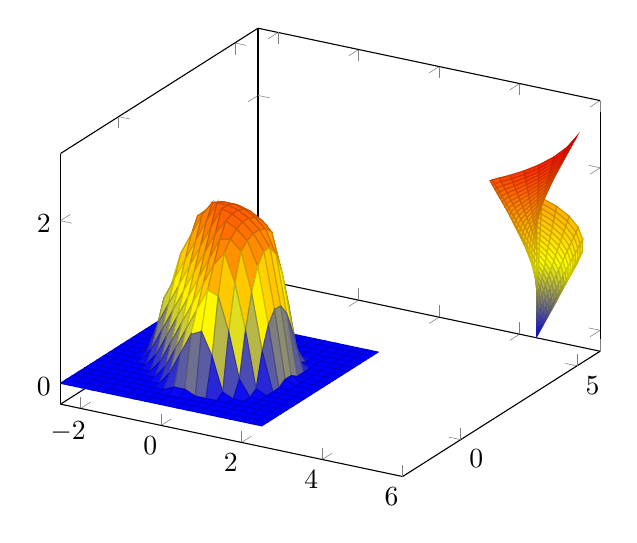
\begin{tikzpicture}
  \begin{axis}[view={30}{30}]

    % Mude os valores de samples para que o gráfico fica mais detalhado
    \addplot3[surf,domain=-2.5:2.5, domain y=-2.5:2.5,
    samples=20, samples y=20]
    % Aqui tem uma função de x e y, gerando o gráfico z=f(x,y).
    % { f(x,y) };
    { max( min( 3-x^2-y^2,
    sqrt( max(4-x^2-y^2, 0) ),
    2 + x + y), 0) };

    % O uso do mínimo acima faz com que seja a parte de baixo
    % de todas as função acima.

    % O uso do máximo dentro do sqrt é para que não tire raiz de negativo.
    % O uso do máximo é para cortar em alguma altura.

    % Uma curva paramétrica
%   \addplot3[black,domain=0:4,samples=30, samples y=0]
%     % (x, y, z); - Em função de x
%     ( { 2*cos(deg(4*x)) }, { 2*sin(deg(4*x)) }, { 5-x } );

    % Uma superfície paramétrica
    \addplot3[surf,domain=0:1, domain y=0:3.14, samples=20, samples y=20]
      % (x, y, z); - Em função de x e y
    ( { x*cos(deg(2*y)) + 5 }, { x*sin(deg(2*y)) + 5 }, { x + y/2 });
  \end{axis}
\end{tikzpicture}
\end{document}
